\documentclass[11pt]{article}
\usepackage{amsmath,amssymb}
\usepackage{graphicx}
\usepackage{array}
\usepackage{changes}
\usepackage{natbib}
\graphicspath{ {/Users/kennedy/Desktop} }
\usepackage[margin=1in]{geometry}
\usepackage[margin=1cm]{caption}
\usepackage[parfill]{parskip}  
\usepackage{gensymb}
\title{Notes on this SPAC implementation\large}
\author{Daniel Kennedy - djk2120@columbia.edu 
}

\begin{document}
\maketitle

\section{Introduction}

\clearpage
\section{Model description}

\subsection{Plant Water Supply Equations}

The basic Darcy flux is described by:

\begin{equation}
q = -\int_{\psi_{soil}}^{\psi_{leaf}}{k\left(\psi\right)d\psi}
\end{equation}

And we adopt a simple linear conductance attenuation parameterization:

\begin{equation}
k(\psi) = \dfrac{\psi - p_2}{p_1 - p_2} \cdot k_\text{max}
\end{equation}

Solve the integral and define $f_k$:

\begin{equation}
q = -k_\text{max}\cdot f_k\left(\Psi_L,\Psi_s\right) \cdot \left(\psi_L-\psi_s\right)
\end{equation}

\begin{equation}
f_k = \dfrac{\dfrac{1}{2} \left(\psi_L+\psi_s\right) - p_2}{p_1 - p_2} \in \left[0,1\right]
\end{equation}


\clearpage
\subsection{Plant Water Demand Equations}
\begin{equation}
T = T_\text{max}\cdot f_T
\end{equation}

\begin{equation}
f_T = \dfrac{\psi_L - p_4}{p_3 - p_4} \in \left[0,1\right]
\end{equation}

\clearpage
\subsection{Solution}

We solve for leaf water potential and transpiration by requiring that: 
\begin{equation}
T = q
\end{equation}

\begin{figure}[h]
\centering
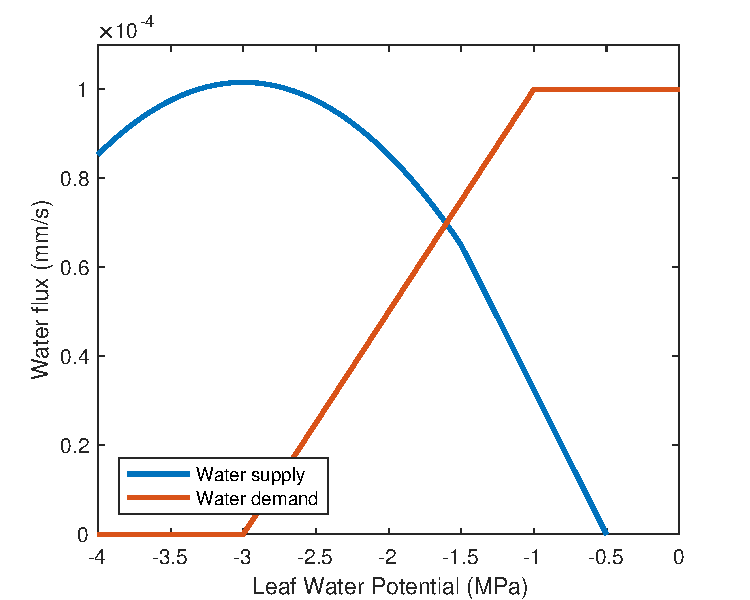
\includegraphics[width=25pc]{../figs/spac_solution}
\caption{The solution for $\Psi_L$ occurs where the two curves intersect.}
\label{fig:soln}
\end{figure}

Because transpiration decreases with decreasing $\Psi_L$ and sap flux increases, we can usually find a satisfactory solution. There are two potential issues:

\begin{enumerate}
\item The curves intersect twice.
	\begin{itemize}
	\item This is possible due to the parabolic shape of the sap flux curve.
	\item We want to choose the less negative value of $\Psi_L$ as our solution.
	\item The numerical implementation is designed to minimize the chances that we find the alternate solution.
	\end{itemize}
\item The curves never intersect.
	\begin{itemize}
	\item The sap flux curve can potentially peak and return to zero before there is enough transpiration attenuation to cause the lines to intersect.
	\item This functionality does not comport well with our expectation of vegetation function, but could arise if we pick `bad' parameter values.
	\item In this case, the model will crash, and provide a message that the parameter values may be unrealistic.
	\end{itemize}
\end{enumerate}


\subsection{Bucket}

Right now the bucket is the simplest it can be. Remove the transpiration each timestep. The bucket is sized according to the effective rooting depth $Z_r$.

\begin{equation}
\theta_1 = \theta_0 - \dfrac{q\Delta t}{Z_r}
\end{equation}

\begin{equation}
\psi_{soil}\left(\theta\right) = \psi_{soil,sat}\left(\dfrac{\theta}{\theta_{sat}}\right)^{-b}
\end{equation}

Do not currently have implementations of:
\begin{itemize}
\item Rain
\item Runoff
\item Drainage
\end{itemize}


\clearpage
\section{Experiments}

\subsection{Experiment 1}
No drainage, no rain. Looking at a 30-day drydown. I'm forcing the model with a constant $T_\text{max}$ of 1e-4 mm/s, which is approximately 4.3 mm/d. 

\begin{figure}[h]
\centering
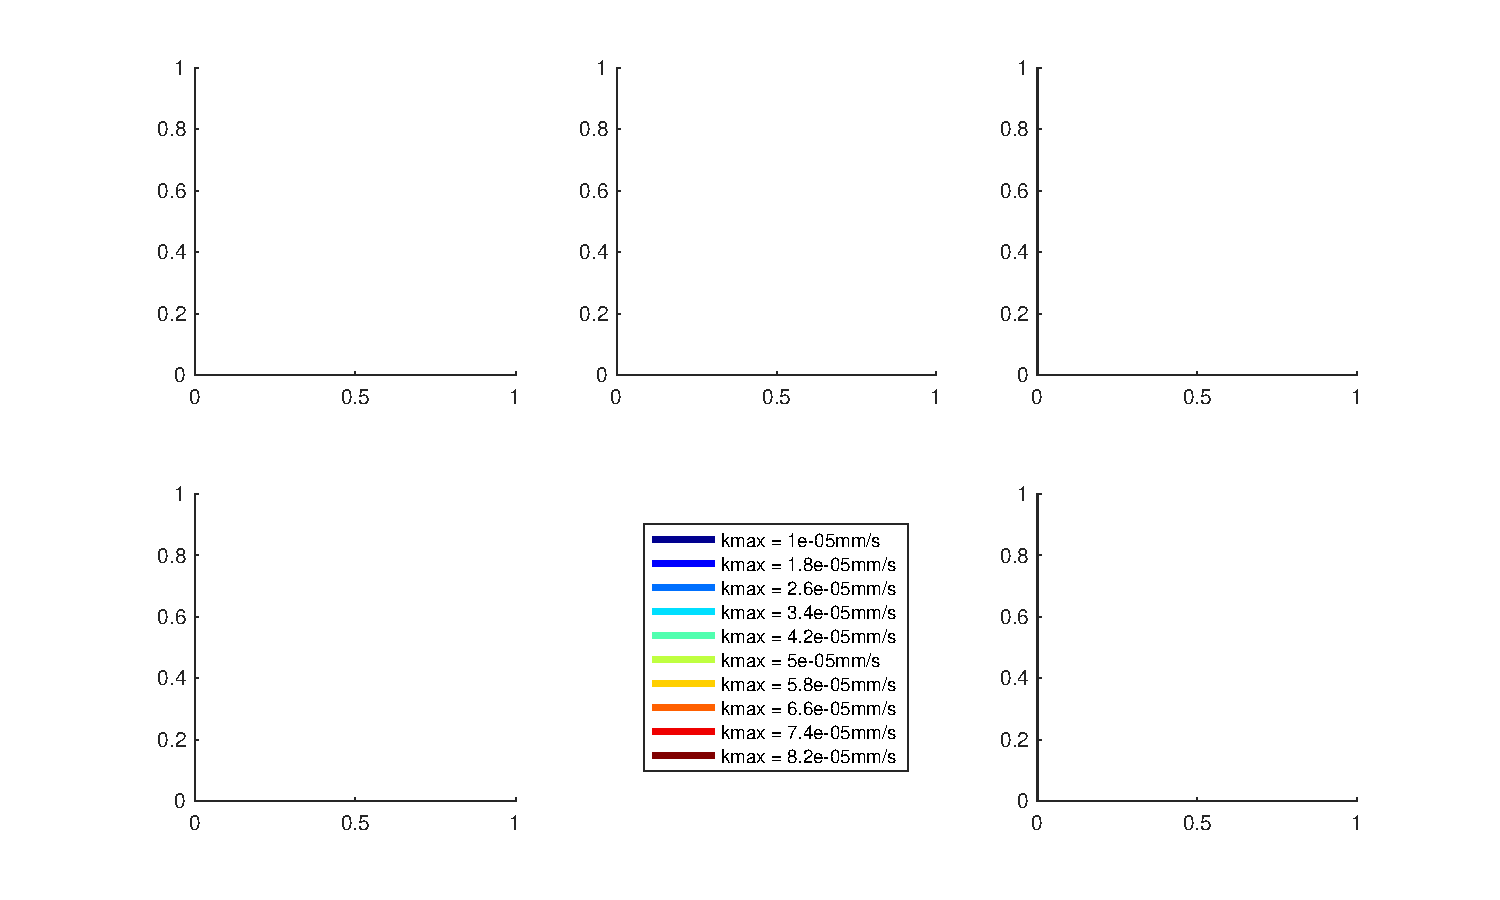
\includegraphics[width=35pc]{../figs/exp1}
\caption{As expected, deeper rooting leads to a longer decay period.}
\label{fig:soln}
\end{figure}





\clearpage
\bibliographystyle{abbrvnat}
\nocite{*}

\bibliography{refs/all}





\end{document}




